% Generated by verification/reference_price_robustness.py
\newcommand{\RefMissMean}{0.108}
\newcommand{\RefWorstMean}{1.195}
\newcommand{\RefWorstPopulation}{1.045}
\newcommand{\RefWorstTail}{2.413}
\newcommand{\RefWorstMCSE}{0.043}

\begingroup\color{black}
\section{Numerical Study and Implementation}
\label{sec:usecase}

\begingroup\color{blue}
We use synthetic experiments to examine how estimated demand informs promotion planning, how price-order dependence affects count-based decisions, and when computational approximations provide useful policies and revenue-loss bounds.
\par\endgroup

\subsection{From estimated demand to a promotion plan}
\label{sec:estimated-cycle}
\label{sec:promotion-budget-numerics}

Consider a monthly access service with regular price \(p^H=9.99\), promotional price \(p^L=5.99\), and active ages \(a=0,\ldots,4\). Market share follows
\[
 M_a(p_t,y_{a,t})=\alpha_a+\beta_a(d_t+y_{a,t}).
\]
Current and remembered promotions have the same age-specific effect, with no current-price response at age zero.

We simulate 400 independent groups over 24 measured months using randomized price histories and binomial purchases. We estimate the age-specific intercepts and slopes by cohort-size-weighted least squares on 300 groups and reserve 100 for validation.

\begingroup\color{blue}
Every estimated \(F_b\) is concave, so the structural results reduce optimization to the finite balanced-frequency search. This selects \(\rho=1/2\), implemented by \(HL\). Under true demand, this policy earns \(6.08\%\) more than constant regular pricing, and an exact state-graph certificate verifies global optimality.
\par\endgroup

\begingroup\color{blue}
The selected cycle is stable across repeated samples under this simulation design. All 20 independent replications select \(HL\), and bootstrap resampling selects it in \(99.2\%\) of replications. Relative to observed average revenue in the holdout sample, mean absolute prediction error is \(0.19\%\), with a maximum of \(0.40\%\); these errors include binomial purchase variation. The simulation design, validation results, and optimality checks appear in Section~\ref{app:subscription-validation}.
\par\endgroup

Arrangement also matters at a fixed frequency. Alternation and a single promotion block both use five promotions in ten periods, but alternation earns \(2.32\%\) more. Figure~\ref{fig:subscription-frontier} compares these calendars with constant pricing, separating the effects of arrangement and frequency.

\begin{figure}[ht]
\centering
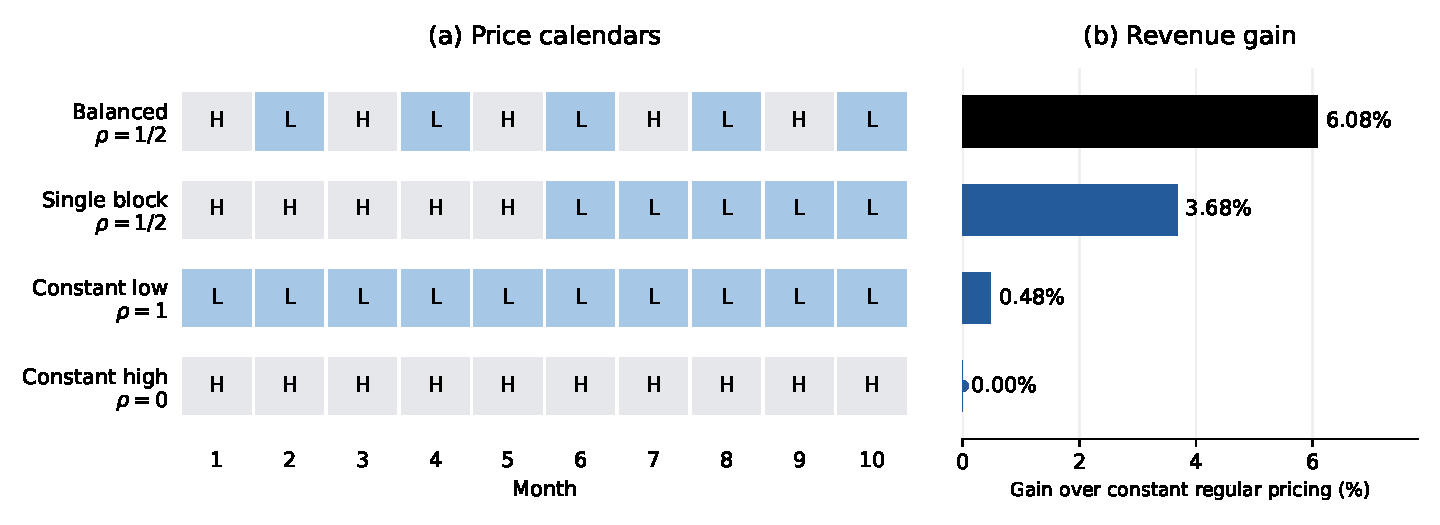
\includegraphics[width=\textwidth]{subscription_usecase_frontier.pdf}
\caption{Ten-month price calendars and revenue gains under true baseline demand. The balanced and single block calendars use the same promotion frequency, isolating the value of arrangement. Constant-price calendars provide frequency benchmarks.}
\label{fig:subscription-frontier}
\end{figure}

To examine promotion budgets, we allow at most \(m\in\{1,2,3,5\}\) promotions in a ten-period cycle. Exact enumeration confirms that each cap binds and a balanced arrangement is optimal. At three promotions, balancing earns \(1.44\%\) more than a single block. The full comparison appears in Table~\ref{tab:promotion-budget-performance} in the supplementary appendix.

\textcolor{blue}{At a fixed frequency, total demand is invariant to arrangement in this affine model, but its time profile changes.} For \(m=2,3,5\), peak demand under balanced arrangements is only \(3.4\%\)--\(7.4\%\) above the mean, compared with \(25\%\)--\(30\%\) under a single block. These smoother profiles suggest potential staffing, capacity, and inventory benefits, whose operating costs are outside the model.

\subsection{Sensitivity to price order}
\label{sec:reference-robustness}

The preceding analysis summarizes remembered promotions by their count. To assess the consequences of discarding price order, we introduce demand with recency-weighted reference prices and asymmetric responses to gains and losses, with and without historical engagement. The experiment contains ten count-based controls and 16 order-dependent cases. The demand specifications and parameter grid appear in Section~\ref{app:numerical-reference}.

\begingroup\color{blue}
The population count model averages true demand within each age, current-price, and past-count cell under the baseline randomized price histories. This benchmark isolates the effect of aggregating histories, while count models estimated from 100 simulated data sets per case introduce sampling variation. Each optimized policy is evaluated under true demand, with revenue loss measured relative to the unrestricted optimum under the full historical model.
\par\endgroup

Across the order-dependent cases, mean estimated-policy revenue loss is \(\RefMissMean\%\). The population count model selects a true optimum in 15 of 16 cases. In the exception, strong gain sensitivity and emphasis on the latest price lead it to select \(HHL\) instead of \(HL\), losing \(\RefWorstPopulation\%\). With estimation, mean loss in this case is \(\RefWorstMean\%\).

Thus the count summary performs well in most tested cases but can miss consequential order effects. In applications, whether recent prices add explanatory power beyond promotion count should be assessed before applying the count-based model. Adding a last-price indicator provides one diagnostic. Detailed results appear in Table~\ref{tab:reference-robustness} in the supplementary appendix.

\subsection{Performance of computational approximations}
\label{sec:approximation-numerics}

\begingroup\color{blue}
We evaluate the two approximations in Section~\ref{sec:approximation} under known demand, without estimation noise, on 1,296 demand functions, including 1,044 with mixed curvature, at \(\mathcal A\in\{4,6,8\}\). The cases cover nonlinear historical responses, effects changing sign across ages, and multiplicative retention. Demand specifications and computational verification details appear in Section~\ref{app:approximation-design}. All losses and bounds below are percentages of the unrestricted full-model optimum; \(1\%\) is the reference tolerance.
\par\endgroup

\paragraph{Balanced and single block policies.}
\begingroup\color{blue}
Choosing the better of the balanced and single block policies limits the maximum loss in the tested instances to \(0.124\%\), compared with \(2.395\%\) for balanced policies alone. The corresponding bound is below \(1\%\) in \(47.0\%\) of cases, but reaches \(32.222\%\) when \(E_B\) and \(E_S\) are comparable. Thus good observed performance can coexist with conservative bounds. Table~\ref{tab:simple-approximation-performance} groups general-demand cases by \(\omega=E_B/(E_B+E_S)\): small values indicate a relatively tighter balanced-policy bound, and large values a relatively tighter single block bound.
\par\endgroup

\begin{table}[ht]
\centering\small
\caption{Maximum revenue loss and its bound (\%). Better selects between balanced and single block policies. Bound is \(100\min\{E_B,E_S\}/\bar R^*\). Column maxima may occur in different cases.}
\label{tab:simple-approximation-performance}
\setlength{\tabcolsep}{5pt}
\begin{tabular}{lrrrrr}
\toprule
Setting & Cases & Balanced & Single block & Better & Bound \\
\midrule
$E_B/(E_B+E_S)\le0.2$ & 201 & 0.071 & 0.048 & 0.000 & 1.317 \\
$0.2<E_B/(E_B+E_S)<0.8$ & 822 & 0.715 & 0.214 & 0.124 & 32.222 \\
$E_B/(E_B+E_S)\ge0.8$ & 201 & 0.000 & 0.000 & 0.000 & 1.333 \\
Multiplicative, mixed & 72 & 2.395 & 0.000 & 0.000 & 13.353 \\
\bottomrule
\end{tabular}

\end{table}

\paragraph{Memory truncation.}
\begingroup\color{blue}
Truncation is most effective when older cohorts contribute little to demand. We optimize every \(J=0,\ldots,\mathcal A-1\) and evaluate each selected policy under full demand. General demand uses the compatible-range midpoint; multiplicative demand omits older survival factors.
\par\endgroup

At \(J=2\), four past-price states replace 16, 64, or 256. Under general demand, the maximum loss is \(0.133\%\) with rapidly fading activity (\(q=0.4\)), but reaches \(6.667\%\) when activity persists (\(q\ge0.95\)). Multiplicative factor omission loses up to \(19.184\%\), illustrating the consequences of overstating older-cohort survival. Detailed comparisons appear in Table~\ref{tab:truncation-performance} in the supplementary appendix.

Figure~\ref{fig:approximation-bounds} distinguishes the memory needed for good policy performance from that needed to certify it. Fading activity permits shorter histories, whereas persistent activity can require the full history to meet the \(1\%\) guarantee. When truncation provides a useful upper bound, it also supplies the complementary certificate for simple policies described in Section~\ref{sec:general-truncation}.

\begin{figure}[!htbp]
\centering
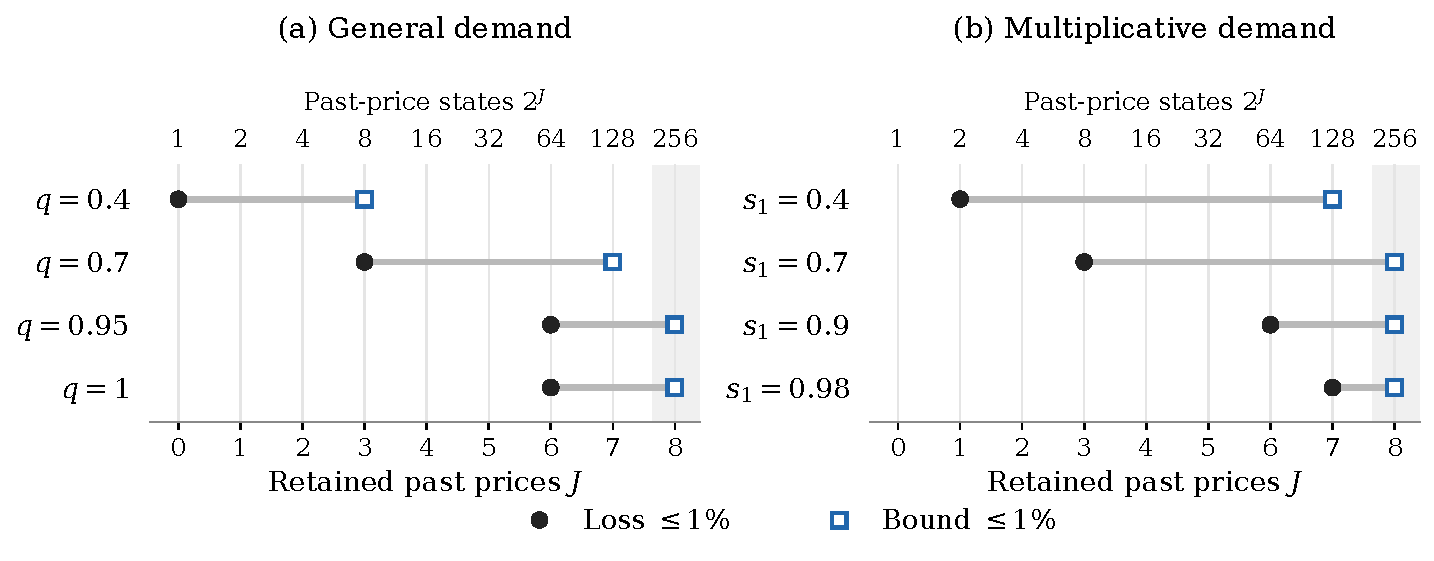
\includegraphics[width=0.96\textwidth]{approximation_bounds.pdf}
\caption{Minimum retained memory at \(\mathcal A=8\) needed to keep revenue loss or its bound at or below \(1\%\). Filled circles and open squares show the respective cutoffs, using maxima over the remaining parameters. Panel (a) covers general demand; panel (b) covers multiplicative factor omission. Upper axes report the corresponding \(2^J\) past-price states.}
\label{fig:approximation-bounds}
\end{figure}

For implementation, demand estimation should be accompanied by checks of order dependence and the stability of the shape conditions. Candidate policies should then be evaluated under the original demand model, with a revenue-loss certificate where available and a demand-profile comparison against operating constraints.
\FloatBarrier
\par\endgroup
